\chapter{Color}

During this chapter, we will explore the concept of color. In order to do so, we firstly need to understand what ``light'' is. Light is a form of electromagnetic radiation, which are two perpendicular transverse waves that propagate through space. These waves consist of two components:
\begin{itemize}
    \item The electric field wave, which oscillates in a plane perpendicular to the direction of propagation.
    \item The magnetic field wave, which also oscillates in a plane perpendicular to the direction of propagation, but is perpendicular to the electric field wave.
\end{itemize}
The last degree of freedom is the polarization of the light, which describes the orientation of the electric field wave. A really important property of light is its wavelength, which divides the electromagnetic spectrum into different regions, from radio waves (long wavelength, less energy) to gamma rays (short wavelength, more energy). The visible spectrum, which is the range of wavelengths that human eyes can perceive, ranges from approximately $\unit{380}{nm}$ (violet) to $\unit{750}{nm}$ (red). The light we perceive is actually a superposition of different wavelengths of light, called a \emph{spectral energy distribution} (represented as a function of wavelength vs. intensity).

Once we have understood what light is, we can define color as the perception of light by the human eye (which will be explained in detail in the next section). The color we percieve depends on the type of object we are looking at:
\begin{itemize}
    \item If the object is a light source, the color we perceive is determined by the spectral energy distribution of the light emitted by the source.
    \item If the object is a non-light source, the color we perceive is determined by the spectral energy distribution of the light reflected by the object. Of all the incoming wavelengths of light that hit the object, some are absorbed (and maybe converted to heat) and some are reflected. The reflected wavelengths are the ones that determine the color we perceive.
\end{itemize}

\section{Technical Color Models}

For biological purposes, colors are defined by a superposition of three primary colors, which are red, green, and blue (as if they were the usual base of $\bb{R}^3$). These three colors (and no other) were chosen because of the three type of cone cells in the human eye (explained in the following section). The similarity between these three primary colors and the three dimensions of a vector space is represented in the RGB color cube in Figure~\ref{fig:color_cube}. Each vertex of the cube represents a color, where the coordinates of the vertex correspond to the intensity of red, green, and blue components.
\begin{figure}
    \centering
    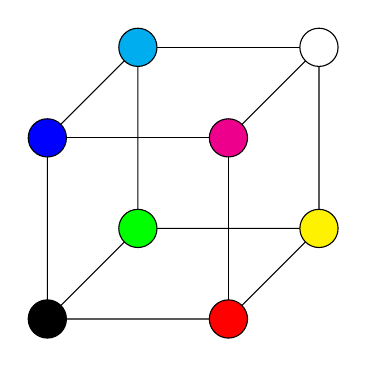
\begin{tikzpicture}[x={(1cm,0cm)}, y={(0.5cm,0.5cm)}, z={(0cm,1cm)}, scale=2.3]
        
        \draw (0, 0, 0) -- (1, 0, 0) -- (1, 1, 0) -- (0, 1, 0) -- cycle;
        \draw (0, 0, 0) -- (0, 0, 1) -- (0, 1, 1) -- (0, 1, 0);
        \draw (1, 0, 0) -- (1, 0, 1) -- (0, 0, 1);
        \draw (1, 1, 0) -- (1, 1, 1) -- (1, 0, 1);
        \draw (0, 1, 1) -- (1, 1, 1);
        
        \draw[fill=black] (0, 0, 0) circle (3pt);
        \draw[fill=red] (1, 0, 0) circle (3pt);
        \draw[fill=green] (0, 1, 0) circle (3pt);
        \draw[fill=blue] (0, 0, 1) circle (3pt);

        \draw[fill=yellow] (1, 1, 0) circle (3pt);
        \draw[fill=cyan] (0, 1, 1) circle (3pt);
        \draw[fill=magenta] (1, 0, 1) circle (3pt);
        \draw[fill=white] (1, 1, 1) circle (3pt);        
    \end{tikzpicture}
    \caption{The RGB color cube.}
    \label{fig:color_cube}
\end{figure}

\subsection{Additive Color Model: RGB}

This color model is called \emph{additive} because the origin is the absence of color (black), and the colors are created by combining the primary colors (red, green, blue) in different intensities. When all three primary colors are combined at full intensity, we get white.

This model is commonly used in sources of light, such as computer monitors, televisions, and smartphones, where colors are created by emitting light. In all these cases, the origin is black (the absence of light), and the colors are created by adding light from the primary colors.

\subsection{Subtractive Color Model: CMY}

This color model is called \emph{subtractive} because the origin is the presence of all colors (white), and the colors are created by mixing the secondary colors (cyan, magenta, yellow) in different intensities. This is done because each of the secondary colors absorbs (or subtracts) one of the primary colors (the one that is not present in the secondary color; the one opposite to it in the RGB color cube):
\begin{itemize}
    \item Cyan (which is in fact a mixture of green and blue) absorbs red.
    \item Magenta (which is in fact a mixture of red and blue) absorbs green.
    \item Yellow (which is in fact a mixture of red and green) absorbs blue.
\end{itemize}

Therefore, when all three secondary colors are combined at full intensity, we get black (the absence of light). This model is commonly used in printing, where the source is a non-light source (the paper) that reflects all the incoming light (white), and the colors are created by subtracting light. The conversion between the RGB and CMY color models is straightforward, as they are complementary to each other:
\begin{align*}
    (R, G, B) &= 1 - (C, M, Y) \\
    (C, M, Y) &= 1 - (R, G, B)
\end{align*}

\subsubsection{CMYK Color Model}

The CMYK color model is an extension of the CMY color model, where the K component stands for ``key'' (black)\footnote{The letter ``B'' is already used for blue in the RGB color model, so we use ``K'' to avoid confusion.}. The reason for adding the K component is that the pigments in real life are not perfect, and when we mix the three secondary colors (cyan, magenta, yellow) at full intensity, we get a dark brown color instead of black. In addition, creating a black ink is much cheaper than creating a black color by mixing the three secondary colors, so it is more efficient to use a separate black ink.

As black absorves all the incoming light, the common conversion between the RGB and CMYK color models is as follows:
\begin{align*}
    K &= \min\{1-R, 1-G, 1-B\} \\
    (C, M, Y) &= 1-(R, G, B) - K
\end{align*}
That way, we reduce the amount of expensive $(C, M, Y)$ ink used, even not using one of them at all (the one that corresponds to the minimum of $1-R$, $1-G$, and $1-B$).

\section{Perceptual Color Models}

% - How we perceive color

\subsection{HSV Color Model}

\subsection{HSL Color Model}

\subsection{YUV Color Model}